%&pdflatex
\documentclass{standalone}
\usepackage{tikz}
\usetikzlibrary{arrows}
\usetikzlibrary{shapes}

\tikzstyle{startstop} = [rectangle, rounded corners, minimum width=3cm, minimum height=1cm,text centered, draw=black, fill=red!30, text width=5cm]
\tikzstyle{io} = [trapezium, trapezium left angle=70, trapezium right angle=110, minimum width=3cm, minimum height=1cm, text centered, draw=black, fill=blue!30,trapezium stretches=true, text width=3cm]
\tikzstyle{process} = [rectangle, minimum width=3cm, minimum height=1cm, text centered, draw=black, fill=orange!30, text width=5cm]
\tikzstyle{decision} = [diamond, minimum width=8cm, minimum height=1cm, text centered, draw=black, fill=green!30, aspect=3]
\tikzstyle{arrow} = [ultra thick,->,>=stealth]
\begin{document}

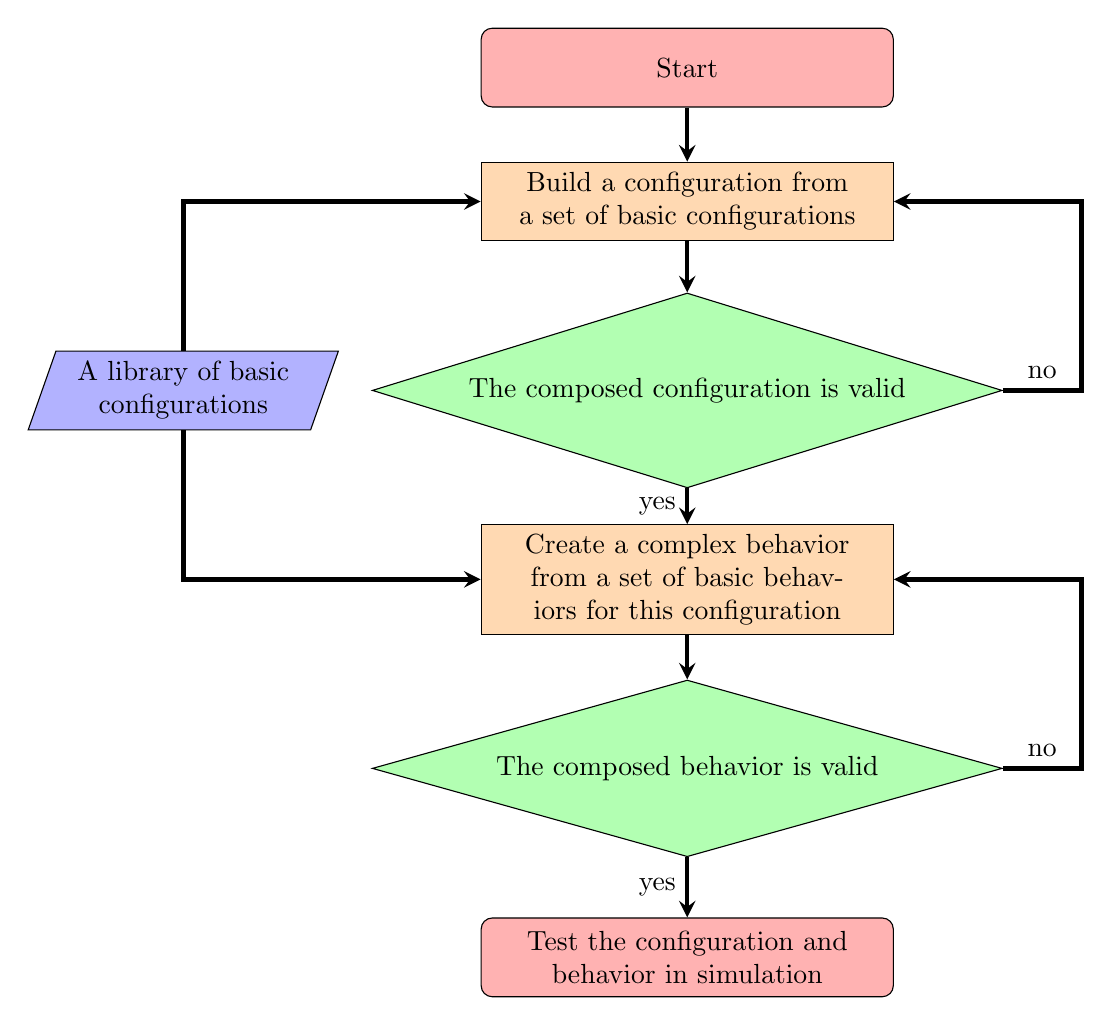
\begin{tikzpicture}[node distance=2.4cm]


\node [process] (build_conf) {Build a configuration from a set of basic configurations};
\node [startstop, above of=build_conf, yshift=-0.7cm] (start) {Start};
\node [decision, below of=build_conf] (verify_conf) {The composed configuration is valid};
\node [io, left of=verify_conf, xshift=-4cm] (library) {A library of  basic configurations};
\node [process, below of=verify_conf] (build_behavior) {Create a complex behavior from a set of basic behaviors for this configuration};
\node [decision, below of=build_behavior] (verify_behavior) {The composed behavior is valid};
\node [startstop, below of=verify_behavior] (sim) {Test the configuration and behavior in simulation};

\draw [arrow] (start) -- (build_conf);
\draw [arrow] (build_conf) -- (verify_conf);
\draw [arrow] (library) |- (build_conf);
\draw [arrow] (library) |- (build_behavior);
\draw [arrow] (verify_conf) -- node[anchor=east] {yes} (build_behavior);
\draw [arrow] (verify_conf) -- node[anchor=south] {no} ([xshift=1cm]verify_conf.east) |- (build_conf.east);
\draw [arrow] (build_behavior) -- (verify_behavior);
\draw [arrow] (verify_behavior) -- node[anchor=east] {yes} (sim);
\draw [arrow] (verify_behavior) -- node[anchor=south] {no} ([xshift=1cm]verify_behavior.east) |- (build_behavior);


\end{tikzpicture}

\end{document}



